% SPDX-License-Identifier: CC-BY-NC-4.0

\documentclass[11pt]{ltjsreport}

\usepackage{geometry}
\usepackage{luatexja-fontspec}
\usepackage{unicode-math}
\usepackage{pgfplots}

\geometry{margin=1in, top=.5in}

\setmainjfont{Noto Sans JP}
\setmainfont{Noto Sans}

\pgfplotsset{compat=1.18}

\setlength{\intextsep}{.5in}

\title{歌声合成ノート}
\author{Jiamu Sun}
\date{2026 年 4 月 3 日}

\begin{document}

\maketitle

\setcounter{chapter}{0}
\chapter{関数}

関数 \( f : A \to B \) とは，任意の \( a \in A \) に対して、\( f(a) \in B \) が
一意に定まる対応である。

\section{変数}

変数とは、対象とする集合の元を表す記号であり、状況に応じて異なる値をとり得るもの
である。

例えば、\( x + 1 \) における \( x \) や、\( f(x) = x^2 \) における \( x \) は変
数である。

\section{定義域}

定義域とは、関数に入力できる値全体の集合である。

例えば、\( f : \mathbb{R} \to \mathbb{R} \) を \( f(x) = x^2 \) で定めるとき、
\( f \) の定義域は \( \mathbb{R} \) である。

\section{値域}

値域とは、関数が実際にとる値全体の集合である。

例えば、\( f : \mathbb{R} \to \mathbb{R} \) を \( f(x) = x^2 \) で定めるとき、
\( f \) の値域は \( \{ y \in \mathbb{R} \mid y \ge 0 \} \) である。

\section{終域}

終域とは、関数の出力先として定められた集合である。また、値域は関数が実際にとる値
全体の集合であるから、値域は終域の部分集合である。

例えば、\( f : \mathbb{R} \to \mathbb{R} \) を \( f(x) = x^2 \) で定めるとき：

\begin{itemize}
   \item 終域は \( \mathbb{R} \)
   \item 値域は \( \{ y \in \mathbb{R} \mid y \ge 0 \} \)
\end{itemize}

\section{対応}

対応とは、定義域の各元に対して、終域の元をただ一つ結び付けることである。

例えば、\( f(x) = x^2 \) は、各実数 \( x \) に対して \( x^2 \) を対応させる関数
である。

\section{記法}

関数は、\( f : A \to B \) のように表す。

これは、関数 \( f \) が集合 \( A \) の各元に対して、集合 \( B \) の元をただ一つ
対応させることを表す。

また、\( a \in A \) に対する対応先を \( f(a) \) と書く。

例えば、各実数 \( x \) に対して \( 2x + 1 \) を対応させる関数は、
\[
   f : \mathbb{R} \to \mathbb{R}, \quad x \mapsto 2x + 1
\]
と表す。このとき、\( f(x) = 2x + 1 \) である。

\section{グラフ}

関数のグラフとは、各 \( x \) に対して点 \( (x, f(x)) \) を座標平面上に表したもの
である。

例えば、\( f(x) = 2x + 1 \) のグラフは、点 \( (x, 2x + 1) \) 全体からなる。

\begin{figure}[h]
   \centering
   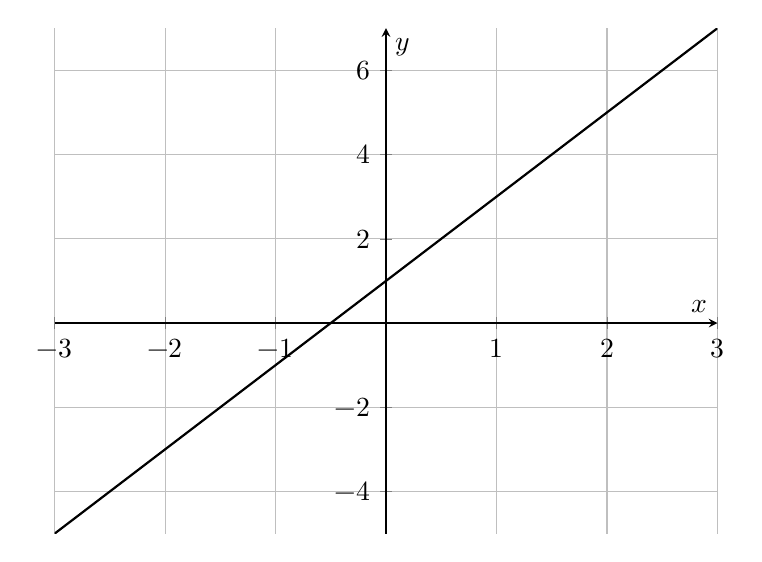
\begin{tikzpicture}
      \begin{axis}[axis lines=middle, xmin=-3, xmax=3, ymin=-5, ymax=7,
                   xlabel={$x$}, ylabel={$y$}, domain=-3:3, samples=2,
                   grid=both, width=10cm, height=8cm]
         \addplot[thick] {2*x + 1};
      \end{axis}
   \end{tikzpicture}
   \caption{\( f(x) = 2x + 1 \)}
\end{figure}

\section{初等関数}

初等関数とは、関数の性質を学ぶときの基礎となる代表的な関数である。

例えば、定数関数、一次関数、二次関数、べき関数、指数関数、対数関数、三角関数など
がある。

\section{合成関数}

合成関数とは、ある関数の出力を別の関数の入力として得られる関数である。

関数 \( f : A \to B \)、\( g : B \to C \) に対して、
\[
   (g \circ f)(x) = g(f(x))
\]
で定まる関数 \( g \circ f : A \to C \) を、\( f \) と \( g \) の合成関数という。

例えば、\( f(x) = 2x + 1 \)、\( g(x) = x^2 \) とするとき、
\[
   (g \circ f)(x) = g(f(x)) = (2x + 1)^2
\]
である。

\section{逆関数}

逆関数とは、ある関数の対応を逆にした関数である。

関数 \( f : A \to B \) に対して、任意の \( b \in B \) に対し \( f(a) = b \) を満
たす \( a \in A \) がただ一つ存在するとき、
\[
   f^{-1}(b) = a
\]
で定まる関数 \( f^{-1} : B \to A \) を \( f \) の逆関数という。

例えば、\( f(x) = 2x + 1 \) とするとき、
\[
   f^{-1}(x) = \frac{x - 1}{2}
\]
である。

\section{単射}

関数の単射とは、異なる入力が必ず異なる出力に対応する性質である。

関数 \( f : A \to B \) に対して、任意の \( a_1, a_2 \in A \) について
\[
   f(a_1) = f(a_2) \implies a_1 = a_2
\]
が成り立つとき、\( f \) は単射であるという。

例えば、\( f : \mathbb{R} \to \mathbb{R} \) を \( f(x) = 2x + 1 \) で定めると
き、\( f \) は単射である。

\section{全射}

関数の全射とは、終域のすべての元が少なくとも一つの入力から得られる性質である。

関数 \( f : A \to B \) に対して、任意の \( b \in B \) に対し、
\[
   f(a) = b
\]
を満たす \( a \in A \) が存在するとき、\( f \) は全射であるという。

例えば、\( f : \mathbb{R} \to \mathbb{R} \) を \( f(x) = x^3 \) で定めるとき、
\( f \) は全射である。

\section{全単射}

関数の全単射とは、単射でもあり全射でもある性質である。

関数 \( f : A \to B \) が全単射であるとき、\( A \) の各元と \( B \) の各元は一対
一に対応する。

例えば、\( f : \mathbb{R} \to \mathbb{R} \) を \( f(x) = 2x + 1 \) で定めると
き、\( f \) は全単射である。

\section{奇関数}

関数の奇関数とは、入力の符号を反転させると、出力の符号も反転する関数である。

定義域が \( x \in A \implies -x \in A \) を満たすとき、関数
\( f : A \to \mathbb{R} \) に対して
\[
   f(-x) = -f(x)
\]
が任意の \( x \in A \) で成り立つならば、\( f \) は奇関数であるという。

例えば、\( f(x) = x^3 \) や \( f(x) = \sin x \) は奇関数である。

\section{偶関数}

関数の偶関数とは、入力の符号を反転させても、出力が変わらない関数である。

定義域が \( x \in A \implies -x \in A \) を満たすとき、関数
\( f : A \to \mathbb{R} \) に対して
\[
   f(-x) = f(x)
\]
が任意の \( x \in A \) で成り立つならば、\( f \) は偶関数であるという。

例えば、\( f(x) = x^2 \) や \( f(x) = \cos x \) は偶関数である。

\section{周期性}

関数の周期性とは、ある長さだけ入力をずらしても、出力が変わらない性質である。

関数 \( f \) に対して、ある正の数 \( T > 0 \) が存在し、
\[
   f(x + T) = f(x)
\]
が成り立つとき、\( f \) は周期 \( T \) をもつという。

例えば、\( f(x) = \sin x \) や \( f(x) = \cos x \) は、周期 \( 2\pi \) をもつ。

\section{単調性}

関数の単調性とは、入力の大小に対して出力の大小関係が保たれる性質である。

区間 \( I \) 上で定義された関数 \( f \) に対して、任意の \( x, y \in I \) が
\( x < y \) を満たすとき、
\[
   f(x) \le f(y)
\]
が成り立つならば、\( f \) は \( I \) 上で単調増加であるという。

また、
\[
   f(x) \ge f(y)
\]
が成り立つならば、\( f \) は \( I \) 上で単調減少であるという。

例えば、\( f(x) = x^2 \) は区間 \( [0, \infty) \) 上で単調増加である。

\section{有界性}

関数の有界性とは、関数の値がある範囲を超えない性質である。

関数 \( f : A \to \mathbb{R} \) に対して、ある実数 \( M \) が存在し、
\[
   f(x) \le M
\]
が任意の \( x \in A \) で成り立つとき、\( f \) は上に有界であるという。

同様に、ある実数 \( m \) が存在し、
\[
   f(x) \ge m
\]
が任意の \( x \in A \) で成り立つとき、\( f \) は下に有界であるという。

例えば、\( f(x) = \sin x \) は
\[
   -1 \le \sin x \le 1
\]
を満たすから、有界である。

\section{対称性}

関数の対称性とは、関数のグラフがある直線や点に関して変わらない性質である。

例えば、偶関数のグラフは \( y \) 軸に関して対称であり、奇関数のグラフは原点に関
して対称である。

実際に、\( f(x) = x^2 \) のグラフは \( y \) 軸対称であり、\( f(x) = x^3 \) のグ
ラフは原点対称である。

\section{区分的定義}

関数の区分的定義とは、入力の条件ごとに異なる式で定める関数の定義方法である。

例えば、絶対値関数は
\[
   f(x) =
   \begin{cases}
      x  & (x \ge 0) \\
      -x & (x < 0)
   \end{cases}
\]
のように定義できる。

このように、場合ごとに式を分けて定める関数を、区分的に定義された関数という。

\end{document}
